\section{Hippocampus} \label{sec: Hippocampus}
The hippocampus is located in the brain and part of an old area called the archicortex. It is named after the greek word for seahorse, because it has the shape of one (\figref{\ref{wrapfig: Hippocampus and seahorse}}). This brain area can be divided into three parts: the dentate gyrus, the cornu ammonis and the subiculum~\cite{ORFrHa20CCN, GarzorzStark18BN}.

\begin{wrapfigure}{r}{0.35\textwidth}
	\centering
		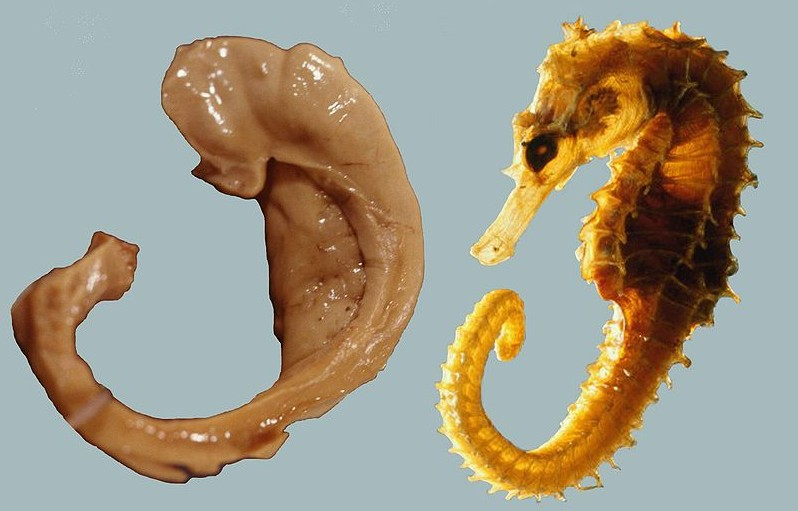
\includegraphics[width=0.35\textwidth]{Hippocampus_and_seahorse.jpg}
	\caption{Hippocampus and seahorse~\cite{Seress10H}} % TODO Besser formatieren oder entfernen
	\label{wrapfig: Hippocampus and seahorse}
\end{wrapfigure}
The hippocampus plays a fundamental role in forming new memories (not preserving them, which is done across the brain) and is highly capable of learning new information fast. Regarding its functions, one was already mentioned: It is the key area when it comes to establishing new memories. Patients with a damaged hippocampus, therefore lacking this ability, will lose spatial and temporal orientation. Moreover epilepsy, schizophrenia and Alzheimer's disease are connected to this dysfunctional organ~\cite{Trepel17N}.
The hippocampus is also important in emotional contexts because it is an integral unit of the limbic system~\cite{GarzorzStark18BN}. Another task, and for this thesis the most important one, is navigation/orientation, not just in spatial surroundings, but also in an abstract context, called \cognitiveroom{}. Some examples for abstract contexts are: Danger of animals based on their appearance and speed of vehicles based on their weight and engine (\secreff{sec: predictive map theory}). To achieve this skill, two types of cells in the hippocampus are active: place cells and grid cells.
The first one encodes states/positions (one for each cell) and the latter resembles a coordinate system.
\paragraph{Place cells} \label{par: Place cell}
Place cells are irregular distributed across the cognitive room. Their firing is tied to the location of the state, whereby the term location has not always its classic spatial meaning if we navigate in an abstract setting (as mentioned above). The place cell is active in case we encounter the associate state. As seen in \figref{\ref{fig: Rat in maze}}, different place cells (each is color coded) fire at different positions in the parkour \eg turquoise is undoubtedly related to the first arch, meaning its activity spikes while the rat passes by. The remark of the thesis lies on place cells.
\begin{figure}
	\centering
		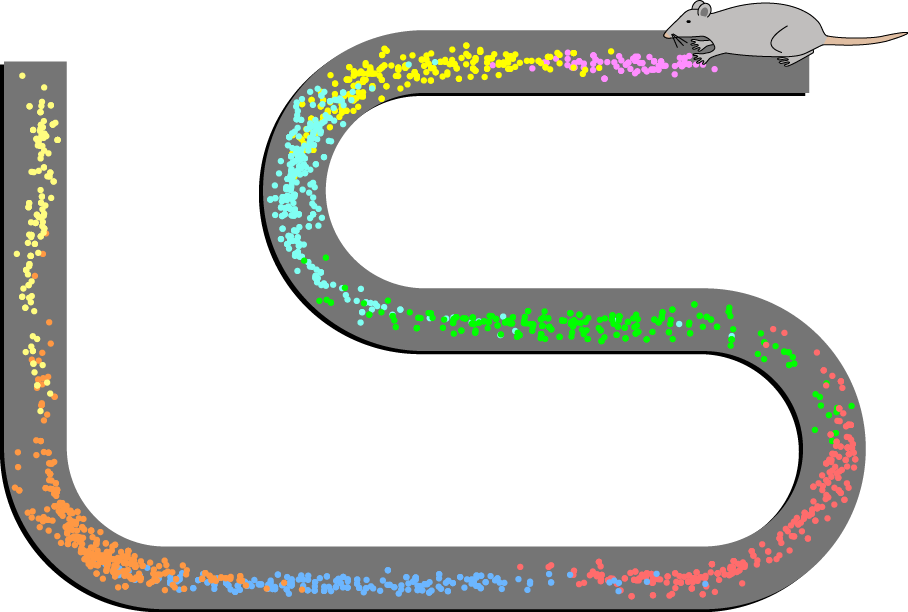
\includegraphics{Ortszelle_Beispiel.png}
	\caption{Activity pattern of color encoded place cell across a maze. Each place cell is exactly related to one distinct position of the corresponding environment \eg turquoise to the first arch. Its activity spikes if the rat walks along the arch~\cite{Stuartlayton13}.}
	\label{fig: Rat in maze}
\end{figure}
%This means in a spatial scenario, where we walk around in a square \TODO[fancyline]{Bild in GeoGebra erstellen mit Quadrat, Brunnen, Baum..., daneben Aktvierungsmuster der Ortszellen} (i.e. with a fountain), it fires irregularly and always then if we are at the position the place cell encodes. In case it resembles the fountain it will fire if we are close to it. \\
\paragraph{Grid cells}
This type of cell can be found in the entorhinal region and satisfies a more general purpose. They are regularly distributed and form a triangular lattice (\figref{\ref{fig: Grid cells}}). It provides raw spatial information in terms of a metric or distance measure the hippocampus integrates with the place cells~\cite{ORFrHa20CCN, BellmundEtAl18NC}.
\begin{figure}
	\centering
		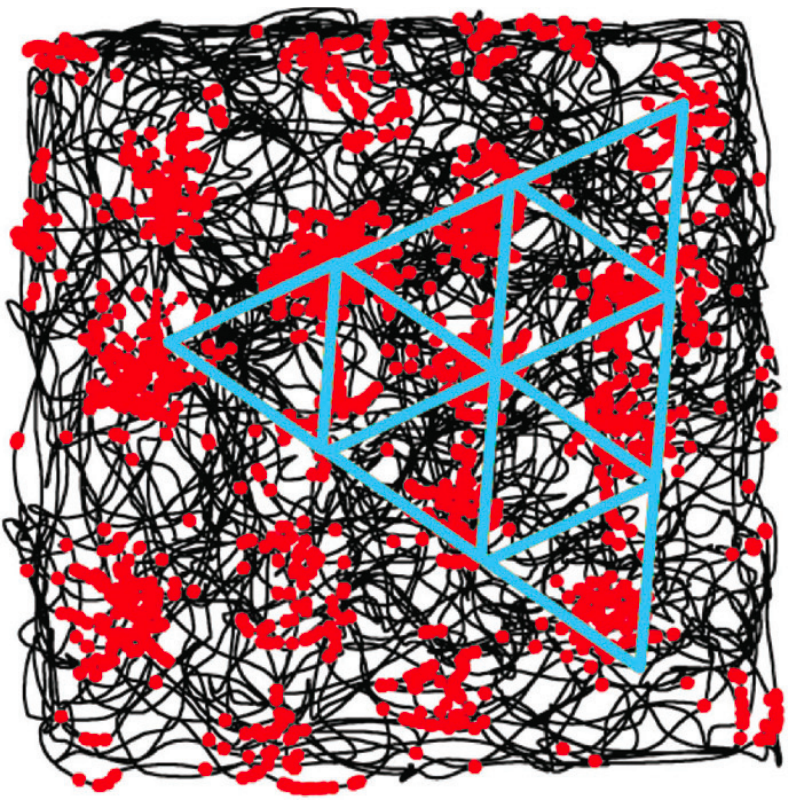
\includegraphics[scale=0.25]{Gitterzelle_Beispiel.png}
	\caption{Sketched path of a rat moving in a square, while tracking firing grid cells. As their name suggests, they form a regular lattice over the space. Hence, they act as coordinate system. The information provided by grid cells is combined with that of the place cells to generate a full picture of the surroundings~\cite{Moser15PGM}.}
	\label{fig: Grid cells}
\end{figure}
